\textbf{a. Accumulator Register}

 Accumulator Register là một thanh ghi 32-bit chịu trách nhiệm lưu trữ các kết quả trung gian từ ALU 
 và cung cấp toán hạng cho các phép toán tiếp theo hoặc ghi ra bộ nhớ.

\begin{figure}[H]
    \centering
    % Đảm bảo file ảnh nằm cùng thư mục với file .tex
    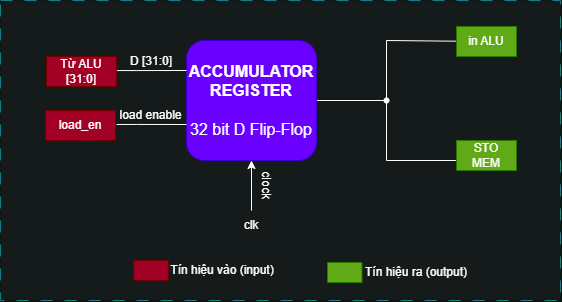
\includegraphics[width=0.65\textwidth]{accum.png} 
    \caption{Sơ đồ khối Accumulator Register}
    \label{fig:accumulator_diagram}
\end{figure}

\textbf{Các thành phần giao tiếp chính:}

\begin{itemize}
    \item \textbf{Tín hiệu vào (Input):}
    \begin{itemize}
        \item \textbf{\texttt{D [31:0]}:} Dữ liệu 32-bit nhận từ đầu ra của khối ALU.
        \item \textbf{\texttt{load\_en}:} Tín hiệu tích cực mức cao cho phép ghi dữ liệu vào Accumulator
        \item \textbf{\texttt{clk}:} Xung clock đồng bộ hóa quá trình.
    \end{itemize}
    
    \item \textbf{Tín hiệu ra (Output): } Tín hiệu rẽ ra hai nhánh 
    \begin{itemize}
        \item \textbf{\texttt{inALU}:} Đi vào khối ALU làm toán hạng đầu vào thứ nhất.
        \item \textbf{\texttt{STO MEM}:} Đi vào bộ đệm và được ghi vào bộ nhớ khi có lệnh STO.
    \end{itemize}
\end{itemize}